% !TEX TS-program = xelatex
% !TEX encoding = UTF-8 Unicode
% !Mode:: "TeX:UTF-8"

\documentclass{resume}
\usepackage{zh_CN-Adobefonts_external} % Simplified Chinese Support using external fonts (./fonts/zh_CN-Adobe/)
%\usepackage{zh_CN-Adobefonts_internal} % Simplified Chinese Support using system fonts
\usepackage{linespacing_fix} % disable extra space before next section
\usepackage{cite}
\usepackage{graphicx}
\usepackage{tabu}
\usepackage{multirow}
\usepackage{color}
\usepackage{hyperref}
\begin{document}
\pagenumbering{gobble} % suppress displaying page number

\Large{
  \begin{tabu}{ c l r }
   \multirow{5}{1in}{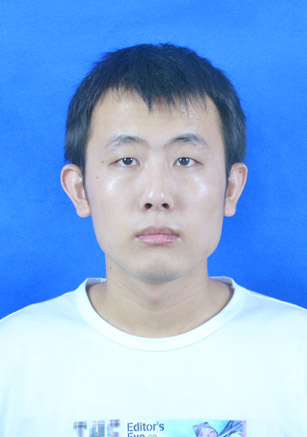
\includegraphics[width=0.88in]{DSC_0804}} & \scshape{丁文东} & \pbar{C/C++}{0.8} \\
    & \email{x007dwd@gmail.com} & \pbar{Python}{0.7} \\
    & \phone{(+86) 153-013-08336} & \pbar{Linux}{0.6} \\
    & \linkedin[bobin]{https://www.linkedin.com/in/bobin-ding-55496b134/} & \pbar{ROS}{0.7} \\
    & \github[github.com/x007dwd]{https://github.com/x007dwd} & \pbar{QT}{0.5}
  \end{tabu}
}

%\name{丁文东}

% \basicInfo{
%   \email{x007dwd@gmail.com} \textperiodcentered\
%   \phone{(+86)153-013-08336} \textperiodcentered\
%   \linkedin[丁文东]{https://www.linkedin.com/in/文东-丁-55496b134}}
  %\linkedin[billryan8]{https://www.linkedin.com/in/billryan8}}
\section{\faGraduationCap\  教育背景}
\datedsubsection{\textbf{中国科学院自动化研究所}, 北京}{\textit{在读博士} \quad 控制理论与控制工程 \quad 2013 -- 至今}
%, 预计 2018 年 6 月毕业
\datedsubsection{\textbf{武汉理工大学}, 武汉, 湖北}{\textit{工学学士}\qquad 电子科学与技术 \quad 2009 -- 2013}


\section{\faUsers\ 项目经历}

\datedsubsection{\textbf{室内移动机器人视觉惯性导航系统}}{程序员:软件部分 \quad 2016.09 -- 至今}
\begin{itemize}\small
  \item 使用DUO 3D双目相机(具备IMU)作为室内移动机器人的视觉系统。在DSO(SLAM系统)系统的基础上加入IMU辅助,提高系统的鲁棒性,并移植到TK1(NVIDIA 嵌入式GPU)系统。
  \item 使用深度网络实现图像的语义分割,辅助并提高视觉定位的精度。
  %\item 在室内安装二维码(AprilTag),搭建基于二维码的视觉室内定位基准系统。
\end{itemize}

\datedsubsection{\textbf{无人机相对定位设计验证平台}}{程序员:软件部分 \quad 2015.11 -- 2016.10}
\begin{itemize}\small
  \item 使用DJI M100四旋翼作为飞行平台,2轴的云台作为视觉系统,TK1 GPU系统作为机载视觉处理系统。软件上通过标志的识别以及特征点提取,测量出无人机的位姿。另外通过PID控制器调整云台,保持标志处在视野的中央。
  \item 使用ROS部署多机(地面站和机载系统)的通信,在机载系统上完成无人机的控制和姿态估计任务,在地面站上进行状态显示和交互。
  \item 通过解决离焦条件下对图像控制点的精确提取,实现对离焦图像鲁棒的相机标定方法。
\end{itemize}

\datedsubsection{\textbf{反射镜表面颗粒物在线监测}}{程序员:软件部分 \quad 2014.07 -- 2015.11}
\begin{itemize}\small
\item 应用散射原理形成暗场成像系统,通过高分辨率相机(6600$\times$4400)获取反射镜(大口径光学系统)表面的颗粒物图像。
\item 颗粒物图像中的背景复杂、信噪比低,为了分割出正确的颗粒物区域,首先提取可能的候选区域,然后通过参考图像对比筛选出正确的颗粒物区域。
\end{itemize}

\datedsubsection{\textbf{机液混合机械臂控制系统}}{毕业设计(驱动、软件) \quad 2013.03 -- 2013.06}
\begin{itemize}\small
  \item 基于ARM的机液混合机械臂控制系统的设计,对液压伺服系统设计控制卡(PCB),液压伺服驱动卡使用stm32作为控制核心,移植uc/os系统完成实验验证。
  \item 研究了机械臂正逆运动学模型及路径规划并进行MATLAB仿真,针对液压系统特性提出模型参考自适应PID,用matlab进行了算法验证,并对系统进行了典型信号的测试。
\end{itemize}
\datedsubsection{\textbf{湖北省大学生电子设计竞赛}}{队长(单片机代码) \quad 2012.03 - 2012.08}
\begin{itemize}\small
  \item 使用DDS芯片完成信号源,产生幅值0-10V带宽0-100KHz的正弦信号。
  \item 信号通过题目要求的模拟模块(频率为4.5KHz的低通滤波器),然后信号经过频率补偿电路,实现电压总增益为1,带宽扩展到100kHz,带内波动小于±10\%、输出噪声电压均方根值小于10mV。
\end{itemize}
\datedsubsection{\textbf{智能电网用户端电能监测系统}}{负责人(ARM及UI代码) \quad 2011.11 -- 2012.04}
\begin{itemize}\small
  \item 该系统为嵌入式的用户端电能质量监控系统,具有电能质量检测、能源功耗计量、电力载波通信、数据自动抄收等功能。
  \item 电能质量检测模块可对用户的现场用电做采样处理,显示质量好坏,做指数评估。能源功耗测量模块可对用电电量、功率、功率因数等重要信息做详尽展示。电力载波通信可将数据使用电力电缆传输,集中汇总。
  \item 下位机使用STM32作为控制核心,完成电能计量,电能质量参数分析。上位机使用QT完成显示及人机交互。
\end{itemize}

\datedsubsection{\textbf{基于等效采样的数字存储示波器}}{负责人(FPGA、单片机软件) \quad 2011.12 -- 2012.03}
\begin{itemize}\small
  \item 该项目使用低成本的低端低速AD实现较高频率的采集和显示,通过信号的程控放大、采样保持、AD转换、FPGA采样保持完成信号的顺序等效采样。
  \item 使用MSP430单片机完成菜单控制和波形等显示。实时采样速率≤1MSa/s,等效采样速率≥200MSa/s,软件触发、触发电平可调。
\end{itemize}



% \datedsubsection{\textbf{分布式科学上网姿势}}{2014年6月 -- 至今}
% \role{Golang, Linux}{个人项目,和富帅糕合作开发}
% \begin{onehalfspacing}
% 分布式负载均衡科学上网姿势, https://github.com/cyfdecyf/cow
% \begin{itemize}
%   \item 修复了连接未正常关闭导致文件描述符耗尽的 bug
%   \item 使用Chord 哈希 URL, 实现稳定可靠地分流
%   \item xxx (尽量使用量化的客观结果)
% \end{itemize}
% \end{onehalfspacing}
%
% \datedsubsection{\textbf{\LaTeX\ 简历模板}}{2015 年5月 -- 至今}
% \role{\LaTeX, Python}{个人项目}
% \begin{onehalfspacing}
% 优雅的 \LaTeX\ 简历模板, https://github.com/billryan/resume
% \begin{itemize}
%   \item 容易定制和扩展
%   \item 完善的 Unicode 字体支持,使用 \XeLaTeX\ 编译
%   \item 支持 FontAwesome 4.5.0
% \end{itemize}
% \end{onehalfspacing}

% Reference Test
%\datedsubsection{\textbf{Paper Title\cite{zaharia2012resilient}}}{May. 2015}
%An xxx optimized for xxx\cite{verma2015large}
%\begin{itemize}
%  \item main contribution
%\end{itemize}
\section{\faCogs\ 成果}
\begin{itemize}\small
  \item {\color{red}W. Ding}, D. Xu, X. Liu, D. Zhang, "A Robust Detection Method of Control Points for Calibration and Measurement with Defocused Images," IEEE Transactions on Instrumentation and Measurement. (SCI, EI Index, Accepted)
  \item {\color{red}W. Ding}, D. Xu, Z. Zhang and D. Zhang, "Particle detection on low contrast image of large aperture optics," 2016 Chinese Control and Decision Conference , Yinchuan, 2016, pp. 5209-5214.(EI index)
  \item {\color{red}W. Ding},, Z. Zhang, D. Zhang, D. Xu, H. Lv, X. Miao, G. Zhou, H. Liu, "An Effective On-line Surface Particles Inspection Instrument for Large Aperture Optical Element," International Journal of Automation and Computing. (EI index, Accepted).
  \item {\color{red}丁文东},徐德,刘希龙,张大朋,移动机器人视觉定位综述, 自动化学报。(EI Index, 在审)
  \item {\color{red}丁文东},张正涛,张大鹏,陶显,史亚莉,吕海兵,苗心向,周国瑞,一种高分辨率显微视觉成像装置与控制方法,专利号: ZL 2014 1 0777930.8,申授权公告日:2017.05.31
  \item 张大朋,张正涛,{\color{red}丁文东},徐德,光学元件表面颗粒物在线监测装置及其在线监测的方法,申请公布号: CN105928949A,申请公布日:2015.09.07
  \item 梁小宇,张纯,{\color{red}丁文东},徐帆. 基于电力载波通信的电能质量监测系统设计[J]. 武汉理工大学学报(信息与管理工程版),2013,(05):659-663.
\end{itemize}
\section{\faCogs\ 技能}
% increase linespacing [parsep=0.5ex]
\begin{itemize}\small
\item 阅读了无人机位姿估计、视觉(惯性)里程计/SLAM、深度网络位姿估计、SLAM语义分析的文献,英语四六级优秀,有较强的英语听说读写能力,熟练使用LaTeX。
\item 撰写CSDN系列博客,\href{http://blog.csdn.net/wendox/article/category/6026381}{玩转四旋翼无人机(35篇)},\href{http://blog.csdn.net/wendox/article/category/6390089}{ROS使用教程(14篇)},\href{http://blog.csdn.net/wendox/article/category/6555599}{SLAM学习(13篇)}。
\item 熟练使用C/C++, Python, Matlab,熟练使用QT,MFC。
\item 熟练Linux下常用指令及C++,Python,ROS开发环境。
\item 理解常用的机器/深度学习,视觉(惯性)SLAM/VO算法(SVO,DSO,ORB SLAM,VINS)。
\item 熟悉常用的SLAM工具 (Sophus、Eigen、G2O),熟练使用OpenCV。
\end{itemize}

\section{\faHeartO\ 获奖情况}
% \datedline{\textit{第一名}, xxx 比赛}{2013 年6 月}
% \datedline{其他奖项}{2015}

\vbox{{\small
  \begin{tabular}{l l}
    研究生阶段 & 中国科学院自动化研究所“三好学生”称号 \\
本科阶段 & \\
2010,2011年国家奖学金 & 2012年武汉理工大学电工电子设计竞赛一等奖\\
2012年 朗坤奖学金	& 2012年湖北省电子设计竞赛二等奖\\
校优秀共青团员、优秀毕业生	&校三好学生标兵\\
  \end{tabular}
}}


% \section{\faInfo\ 其他}
% % increase linespacing [parsep=0.5ex]
% \begin{itemize}[parsep=0.5ex]
%   \item 技术博客: http://blog.csdn.net/wendox
%   \item GitHub: https://github.com/x007dwd
%   \item 语言: 英语 - 熟练(四级 603 六级 555)
% \end{itemize}

%% Reference
%\newpage
%\bibliographystyle{IEEETran}
%\bibliography{mycite}
\end{document}
